\chapter{Edge detection}


\begin{description}
    \item[Edge] \marginnote{Edge}
        Pixel lying in between regions of the image with different intensities.
\end{description}



\section{Gradient thresholding}

\subsection{1D step-edge}
\marginnote{1D step-edge}

In the transition region, the absolute value of the first derivative grows (the absolute value is used as the polarity is not relevant).
By fixing a threshold, an edge can be detected.

\begin{figure}[H]
    \begin{subfigure}{0.4\linewidth}
        \centering
        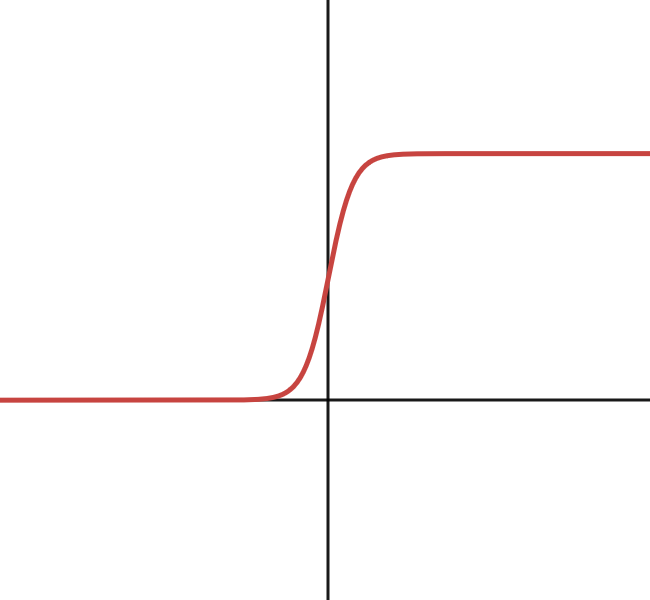
\includegraphics[width=0.5\linewidth]{./img/1d_step_edge_example1.png}
        \caption{Input signal}
    \end{subfigure}
    \begin{subfigure}{0.4\linewidth}
        \centering
        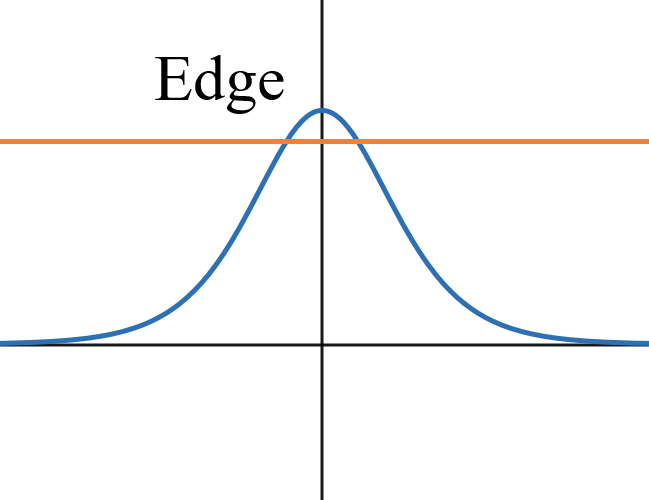
\includegraphics[width=0.5\linewidth]{./img/1d_step_edge_example2.png}
        \caption{Derivative of the signal}
    \end{subfigure}
\end{figure}


\subsection{2D step-edge}
\marginnote{2D step-edge}

In a 2D signal (e.g. an image), the gradient allows to determine the magnitude and the direction of the edge.
\[ 
    \nabla I(x, y) = 
    \begin{pmatrix} \frac{\partial I(x, y)}{\partial x} & \frac{\partial I(x, y)}{\partial y} \end{pmatrix} =
    \begin{pmatrix} \partial_x I & \partial_y I \end{pmatrix}
\]
\[
    \begin{split}
        \text{Magnitude: } & \Vert \nabla I(x, y) \Vert \\
        \text{Direction: } & \arctan\left(\frac{\partial_y I}{\partial_x I}\right) \in [-\frac{\pi}{2}, \frac{\pi}{2}] \\
        \text{Direction and sign: } & \arctan2(\partial_x I, \partial_y I) \in [0, 2\pi] \\
    \end{split}  
\]

\begin{description}
    \item[Discrete gradient approximation] \marginnote{Discrete gradient approximation}
        Approximation of the partial derivatives as a difference.
        \begin{description}
            \item[Backward difference] \marginnote{Backward difference}
                \[ \partial_x I(i, j) \approx I(i, j) - I(i, j-1) \hspace{3em} \partial_y I(i, j) \approx I(i, j) - I(i-1, j) \]


            \item[Forward difference] \marginnote{Forward difference}
                \[ \partial_x I(i, j) \approx I(i, j+1) - I(i, j) \hspace{3em} \partial_y I(i, j) \approx I(i+1, j) - I(i, j) \]

            \begin{remark}
                Forward and backward differences are equivalent to applying two cross-correlations with kernels 
                $\begin{pmatrix} -1 & 1 \end{pmatrix}$ and $\begin{pmatrix} -1 \\ 1 \end{pmatrix}$.
            \end{remark}

            \item[Central difference] \marginnote{Central difference}
                \[ \partial_x I(i, j) \approx I(i, j+1) - I(i, j-1) \hspace{3em} \partial_y I(i, j) \approx I(i+1, j) - I(i-1, j) \]
                
                \begin{remark}
                    Central difference is equivalent to applying two cross-correlations with kernels 
                    $\begin{pmatrix} -1 & 0 & 1 \end{pmatrix}$ and $\begin{pmatrix} -1 \\ 0 \\ 1 \end{pmatrix}$.
                \end{remark}
        \end{description}

    \item[Discete magnitude approximation] \marginnote{Discete magnitude approximation}
        The gradient magnitude can be approximated using the approximated partial derivatives:
        \[ 
            \Vert \nabla I \Vert = \sqrt{(\partial_x I)^2 + (\partial_y I)^2} \hspace{1.5em}
            \Vert \nabla I \Vert_+ = \vert \partial_x I \vert + \vert \partial_y I \vert \hspace{1.5em}
            \Vert \nabla I \Vert_\text{max} = \max(\vert \partial_x I \vert, \vert \partial_y I \vert)
        \]

        Among all, $\Vert \nabla I \Vert_\text{max}$ is the most isotropic (i.e. gives a more consistent response).
        \begin{example}
            Given the following images:
            \[
                E_v = \begin{pmatrix}
                    0 & 0 & h & h \\
                    0 & 0 & h & h \\
                    0 & 0 & h & h \\
                    0 & 0 & h & h \\
                \end{pmatrix}
                \,\,\,
                E_h = \begin{pmatrix}
                    0 & 0 & 0 & 0 \\
                    0 & 0 & 0 & 0 \\
                    h & h & h & h \\
                    h & h & h & h \\
                \end{pmatrix}
                \,\,\,
                E_d = \begin{pmatrix}
                    0 & 0 & 0 & 0 & h \\
                    0 & 0 & 0 & h & h \\
                    0 & 0 & h & h & h \\
                    0 & h & h & h & h \\
                \end{pmatrix}
            \]
            The magnitudes are:
            \begin{center}
                \begin{tabular}{c|ccc}
                    \toprule
                        & $\Vert \nabla I \Vert$ & $\Vert \nabla I \Vert_+$ & $\Vert \nabla I \Vert_\text{max}$ \\
                    \midrule
                    $E_h$ & $h$ & $h$ & $h$ \\
                    $E_v$ & $h$ & $h$ & $h$ \\
                    $E_d$ & $\sqrt{2}h$ & $2h$ & $h$ \\
                    \bottomrule
                \end{tabular}
            \end{center}
        \end{example}
\end{description}

\begin{remark}
    In practice, the signal of an image is not always smooth due to noise. 
    Derivatives amplify noise and are therefore unable to recognize edges.

    Smoothing the signal before computing the derivative allows to reduce the noise but also blurs the edges making it more difficult to localize them.

    A solution is to smooth and differentiate in a single operation by approximating the gradient as a difference of averages.
\end{remark}

\begin{description}
    \item[Smooth derivative] \marginnote{Smooth derivative}
        Compute the approximation of a partial derivative as the difference of the pixels in a given window.
        For instance, considering a window of 3 pixels, the cross-correlation kernels are:
        \[ \frac{1}{3} \begin{pmatrix} -1 & 1 \\ -1 & 1 \\ -1 & 1 \end{pmatrix} \hspace{3em} \frac{1}{3} \begin{pmatrix} -1 & -1 & -1 \\ 1 & 1 & 1 \end{pmatrix} \]

        \begin{description}
            \item[Prewitt operator] \marginnote{Prewitt operator}
                Derivative approximation using central differences.
                The cross-correlation kernels are:
                \[ 
                    \frac{1}{3} \begin{pmatrix} -1 & 0 & 1 \\ -1 & 0 & 1 \\ -1 & 0 & 1 \end{pmatrix} 
                    \hspace{3em} 
                    \frac{1}{3} \begin{pmatrix} -1 & -1 & -1 \\ 0 & 0 & 0 \\ 1 & 1 & 1 \end{pmatrix} 
                \]

            \item[Sobel operator] \marginnote{Sobel operator}
                Prewitt operator where the central pixels have a higher weight.
                The cross-correlation kernels are:
                \[ 
                    \frac{1}{4} \begin{pmatrix} -1 & 0 & 1 \\ -2 & 0 & 2 \\ -1 & 0 & 1 \end{pmatrix} 
                    \hspace{3em} 
                    \frac{1}{4} \begin{pmatrix} -1 & -2 & -1 \\ 0 & 0 & 0 \\ 1 & 2 & 1 \end{pmatrix} 
                \]
        \end{description}
\end{description}

\begin{remark}
    Thresholding is inaccurate as choosing the threshold is not straightforward.
    An image has strong and weak edges. Trying to detect one type might lead to poor detection of the other.

    A better solution is to find a local maxima of the absolute value of the derivatives.
\end{remark}



\section{Non-maxima suppression (NMS)}
\marginnote{Non-maxima suppression (NMS)}

Algorithm that looks for local maxima of the absolute value of the gradient along the gradient direction.

The algorithm works as follows:
\begin{enumerate}
    \item Given a pixel at coordinates $(i, j)$,
        estimate the magnitude $G = \Vert \nabla I(i, j) \Vert$ and the direction $\theta$ of the gradient.
    \item Consider two points $A$ and $B$ along the direction $\theta$ passing through $(i, j)$
        and compute their gradient magnitudes $G_A$ and $G_B$.
    \item Substitute the pixel $(i, j)$ as follows:
        \[ \texttt{NMS}(i, j) = \begin{cases}
            1 & (G > G_A) \land (G > G_B) \text{ (i.e. local maximum)} \\
            0 & \text{otherwise} \\
        \end{cases} \]
\end{enumerate}

\begin{remark}
    After applying NMS, the resulting signal (now composed of 0s and 1s) is converted back to the original gradient magnitudes
    in such a way that pixels 0ed by NMS remain 0 and pixels set at 1 by NMS return to their original value.

    After the conversion, a thresholding step might be applied to filter out unwanted edges that are either due to noise or not relevant.
\end{remark}


\subsection{Linear interpolation}

As there might not be two points $A$ and $B$ along the direction $\theta$ belonging the the discrete pixel grid
and because one doesn't want to consider two points too far from $(i, j)$,
it is possible to use linear interpolation to estimate the gradients of $A$ and $B$ even if off-grid by an offset $\Delta x$:\\
\begin{minipage}{0.6\linewidth}
    \[
        \begin{split}
            G_1 &= \Vert \nabla I(i-1, j) \Vert \hspace{2em} G_2 = \Vert \nabla I(i-1, j+1) \Vert \\
            G_3 &= \Vert \nabla I(i+1, j) \Vert \hspace{2em} G_4 = \Vert \nabla I(i+1, j-1) \Vert \\
        \end{split}
    \]
    \[
        \begin{split}
            G_A &\approx G1 + (G2 - G1)\Delta x \\
            G_B &\approx G3 - (G3 - G4)\Delta x \\
        \end{split}
    \]
\end{minipage}
\begin{minipage}{0.35\linewidth}
    \centering
    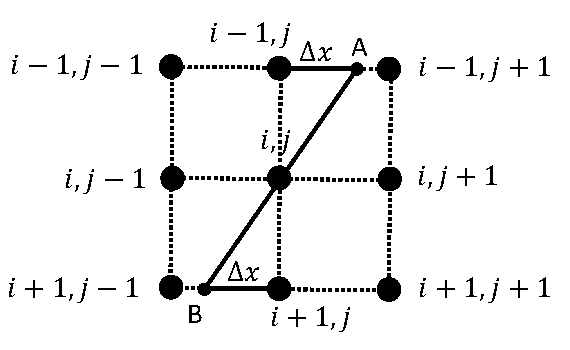
\includegraphics[width=\linewidth]{./img/_nms_interpolation.pdf}
\end{minipage}



\section{Canny's edge detector}

Method based on three criteria:
\begin{descriptionlist}
    \item[Good detection] Correctly detect edges in noisy images.
    \item[Good localization] Minimize the distance between the found edges and the true edges.
    \item[One response to one edge] Detect only one pixel at each true edge.
\end{descriptionlist}

In the 1D case, the optimal operator consists in finding the local extrema of the
signal obtained by convolving the image and the Gaussian first-order derivative. 

Generalized for the 2D case, Canny's edge detector does the following: \marginnote{Canny's edge detector}
\begin{enumerate}
    \item Gaussian smoothing.
    \item Gradient computation.
    \item NMS and thresholding.
\end{enumerate}

It is possible to exploit the convolutions property of being commutative w.r.t. differentiation
and simplify the smoothing and gradient computation:
\[  
    \begin{split}
        \partial_x I(x, y) &= \frac{\partial}{\partial x} ( I(x, y) * G(x, y) ) = I(x, y) * \frac{\partial G(x, y)}{\partial x} \\
        \partial_y I(x, y) &= \frac{\partial}{\partial y} ( I(x, y) * G(x, y) ) = I(x, y) * \frac{\partial G(x, y)}{\partial y}
    \end{split}
\]
By leveraging the separability of a 2D Gaussian ($G(x, y) = G_1(x)G_2(y)$),
the computation can be reduced to 1D convolutions:
\[
    \begin{split}
        \partial_x I(x, y) &= I(x, y) * (G_1'(x)G_2(y)) = (I(x, y) * G_1'(x)) * G_2(y) \\
        \partial_y I(x, y) &= I(x, y) * (G_1(x)G_2'(y)) = (I(x, y) * G_1(x)) * G_2'(y) 
    \end{split}  
\]

\begin{remark}
    When magnitude varies along the object contour, thresholding might remove true edges (edge streaking).
\end{remark}

\begin{description}
    \item[Hysteresis thresholding] \marginnote{Hysteresis thresholding}
        Given a high threshold $T_\text{h}$ and a low threshold $T_\text{l}$,
        depending on its magnitude, a pixel $(i, j)$ can be considered a:
        \begin{descriptionlist}
            \item[Strong edge] $\nabla I(i, j) > T_h$.
            \item[Weak edge] $\nabla I(i, j) > T_l$ and the pixel $(i, j)$ is a neighbor of a strong/weak edge.
        \end{descriptionlist}
        In practice, the algorithm starts from strong edges and "propagates" them.

        \begin{figure}[H]
            \centering
            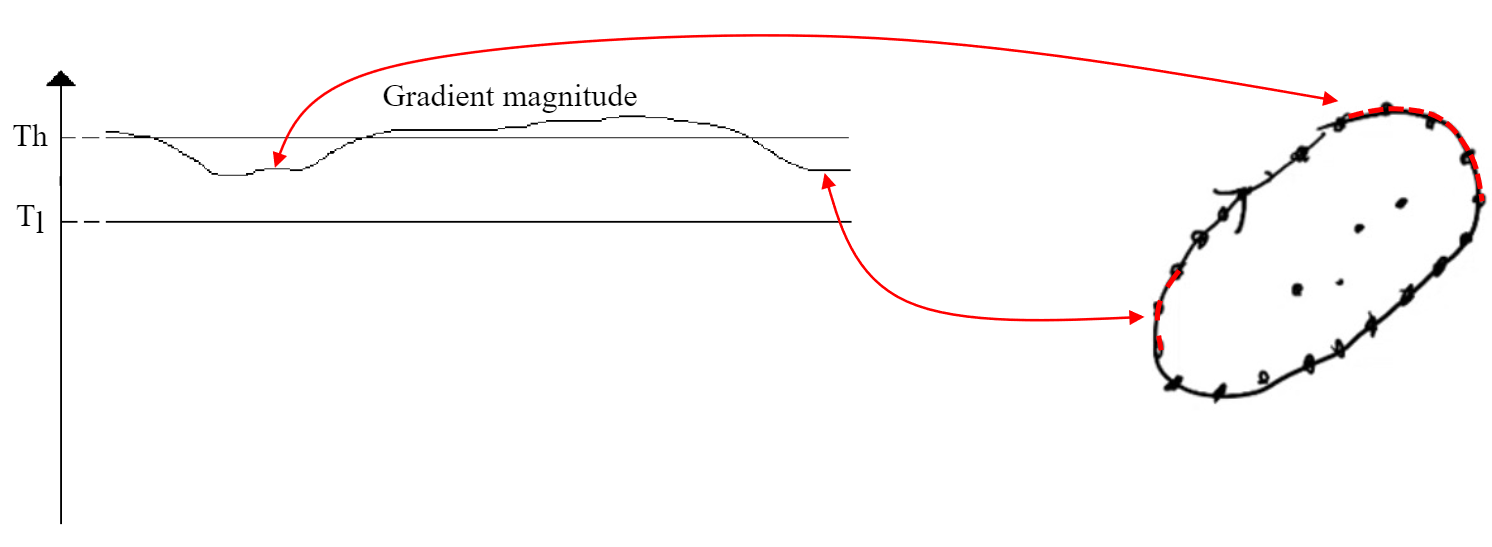
\includegraphics[width=0.5\linewidth]{./img/hysteresis thresholding.png}
            \caption{Application of hysteresis thresholding}
        \end{figure}
\end{description}

\begin{remark}
    The output of Canny's edge detector is not an image with edges but a list of edges.

    Note that if the edges of two objects intersect, this will be recognized as a single edge.
\end{remark}



\section{Zero-crossing edge detector}

\begin{description}
    \item[Zero-crossing edge detector] \marginnote{Zero-crossing}
        Detect edges by finding zero-crossing of the second derivative of the signal.

        \begin{remark}
            A zero-crossing is a point at 0 where the function changes sign.
        \end{remark}

        \begin{remark}
            This approach does not require a threshold anymore but is computationally more expensive.
        \end{remark}

        \begin{figure}[H]
            \centering
            \begin{subfigure}{0.3\linewidth}
                \centering
                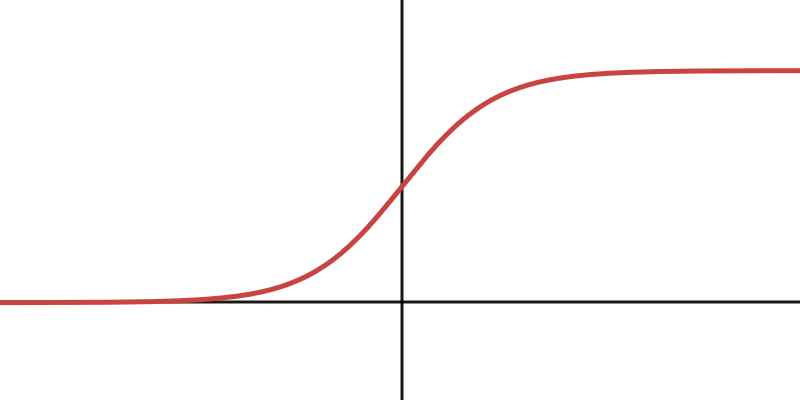
\includegraphics[width=\linewidth]{./img/zero_crossing_example1.png}
                \caption{Input signal}
            \end{subfigure}
            \begin{subfigure}{0.3\linewidth}
                \centering
                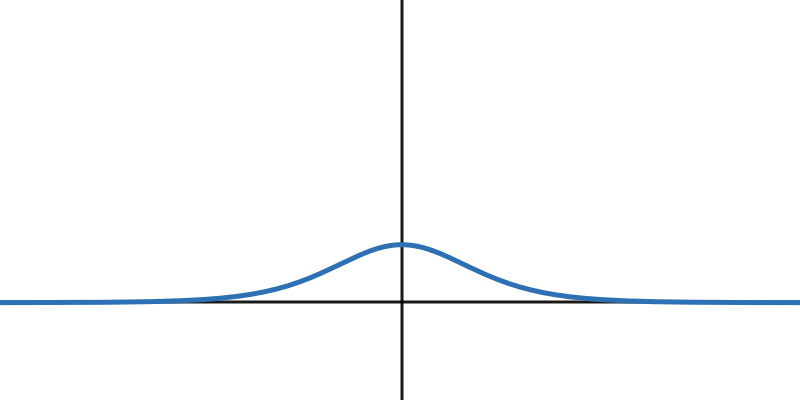
\includegraphics[width=\linewidth]{./img/zero_crossing_example2.png}
                \caption{First-order derivative}
            \end{subfigure}
            \begin{subfigure}{0.3\linewidth}
                \centering
                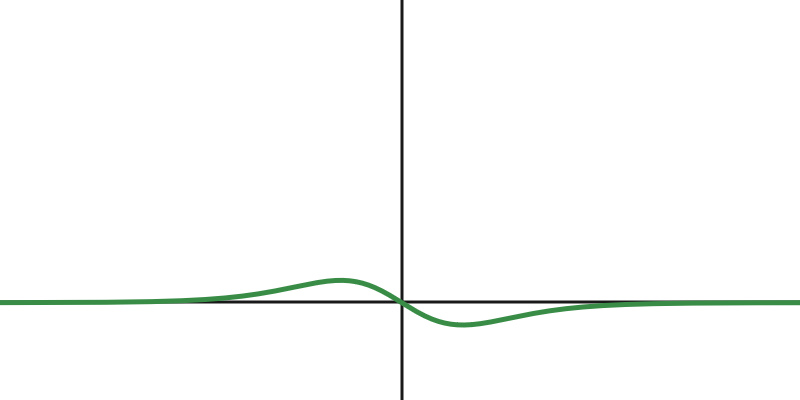
\includegraphics[width=\linewidth]{./img/zero_crossing_example3.png}
                \caption{Second-order derivative}
            \end{subfigure}
        \end{figure}


    \item[Laplacian] \marginnote{Laplacian}
        Approximation of the second-order derivative:
        \[ \nabla^2 I(x, y) \approx \frac{\partial^2 I(x, y)}{\partial x^2} + \frac{\partial^2 I(x, y)}{\partial y^2} = \partial_{x,x} I + \partial_{y, y} I \]


    \item[Discrete Laplacian] \marginnote{Discrete Laplacian}
        Use forward difference to compute first-order derivatives,
        followed by backward difference to compute second-order derivatives.
        \[
            \begin{split}
                \partial_{x,x} I(i, j) &\approx \partial_x I(i, j) - \partial_x I(i, j-1) \\
                    &= \big ( I(i, j+1) - I(i, j) \big) - \big ( I(i, j) - I(i, j-1) \big) \\
                    &= I(i, j+1) - 2I(i, j) + I(i, j-1)
            \end{split}            
        \]
        \[
            \begin{split}
                \partial_{y,y} I(i, j) &\approx \partial_y I(i, j) - \partial_y I(i-1, j) \\
                    &= \big ( I(i+1, j) - I(i, j) \big) - \big ( I(i, j) - I(i-1, j) \big) \\
                    &= I(i+1, j) - 2I(i, j) + I(i-1, j)
            \end{split}            
        \]

        This is equivalent to applying the cross-correlation kernel:
        \[
            \nabla^2 = \begin{pmatrix}
                0 & 1 & 0 \\
                1 & -4 & 1 \\
                0 & 1 & 0 \\
            \end{pmatrix}    
        \]

        \begin{remark}
            It can be shown that zero-crossings of the Laplacian typically lay close to those of the second-order derivative.
        \end{remark}
\end{description}


\subsection{Laplacian of Gaussian (LoG)}

Laplacian of Gaussian (LoG) does the following: \marginnote{Laplacian of Gaussian (LoG)}
\begin{enumerate}
    \item Gaussian smoothing.
    \item Second-order differentiation using the Laplacian filter.
    \item Zero-crossings extraction.
\end{enumerate}

\begin{description}
    \item[Discrete zero-crossing]
        As the image consists of a discrete grid of pixels, finding a zero-crossing as per definition is not always possible.
        Instead, an edge is detected when there is a change of sign in the magnitude.
        The edge pixel can be identified as:
        \begin{itemize}
            \item The pixel where the magnitude is positive.
            \item The pixel where the magnitude is negative.
            \item The pixel where the absolute value of the magnitude is smaller. 
                This is usually the best choice as it is closer to the true zero-crossing.
        \end{itemize}
\end{description}

\begin{remark}
    A final thresholding might still be useful to remove uninteresting edges.
\end{remark}

\begin{remark}
    Smaller values of $\sigma$ of the smoothing operator detect more detailed edges, 
    while higher $\sigma$ captures more general edges.
\end{remark}

\begin{figure}[H]
    \centering
    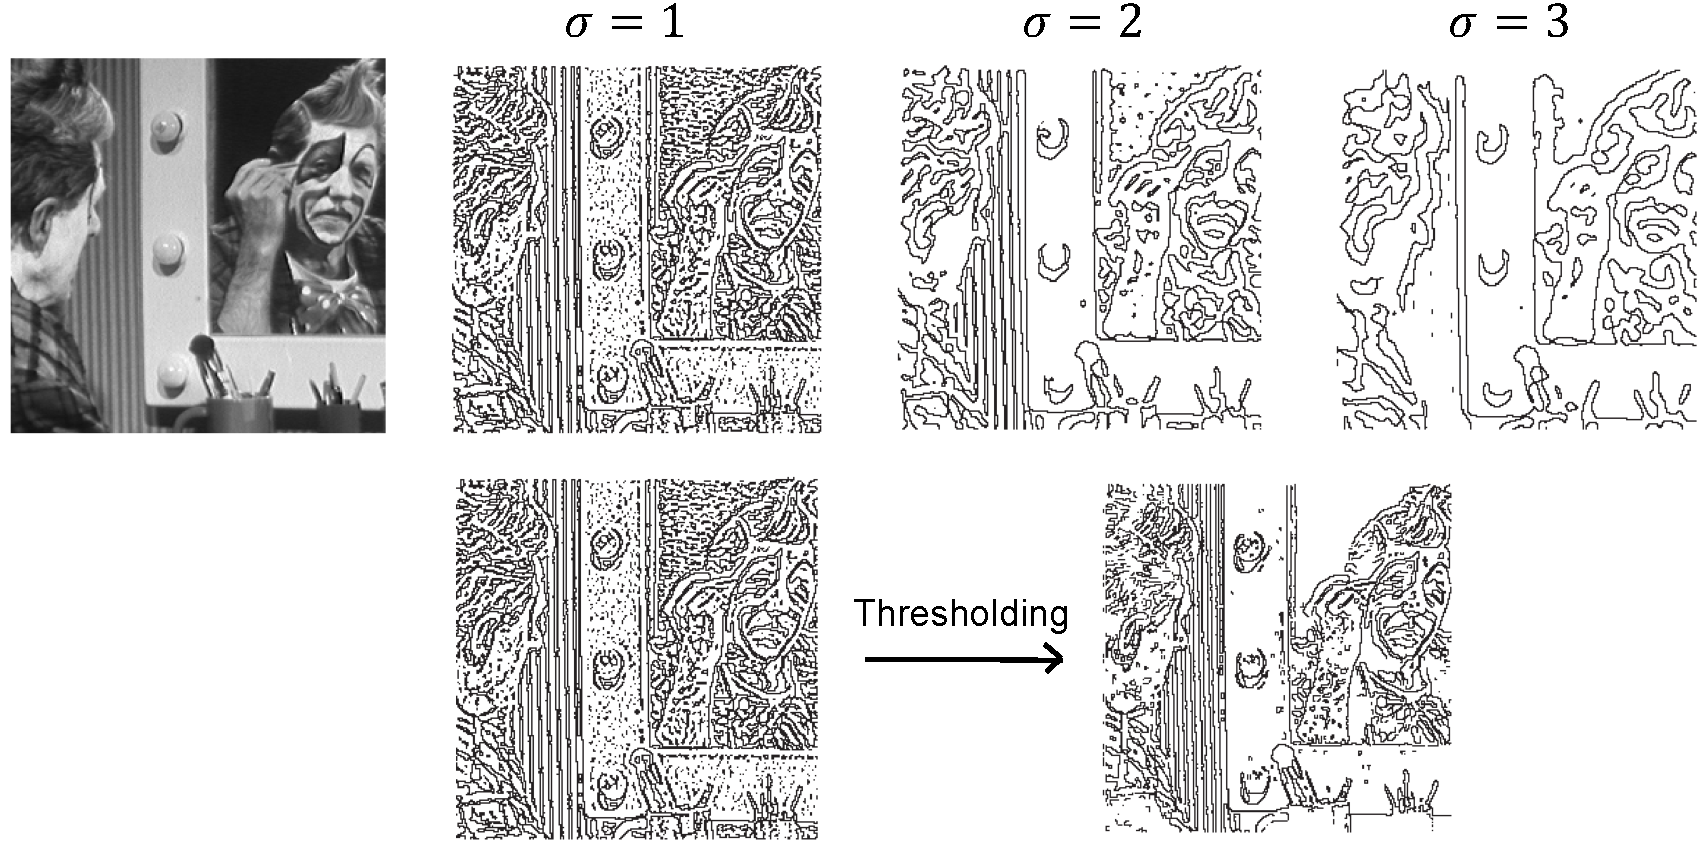
\includegraphics[width=0.8\linewidth]{./img/_example_laplacian_gaussian.pdf}
\end{figure}